\begin{frame}
	\frametitle{El equipo}
	
	Puede que tus primeros juegos los desarrolles de forma individual,
	pero los equipos suelen componerse de:
		
	\begin{columns}[c]
	\column{200pt}	
	
	\begin{block}{Componentes de un equipo}
		\begin{itemize}
			\item Diseñadores
			\item Ingenieros y programadores
			\item Artistas 2D
			\item Artistas 3D
			\item Sonido
			\item Otro equipo: soporte, marketing etc.
		\end{itemize}            
	\end{block}
	
	\column{100pt}
	\begin{center}
	    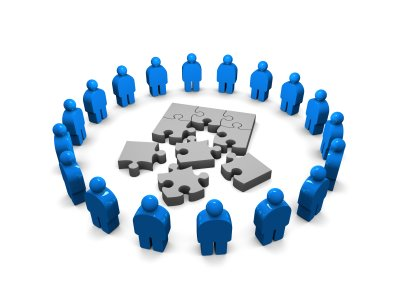
\includegraphics[scale=0.3]{img/collaborate.jpg}
	\end{center}
	
	
	\end{columns}
\end{frame}

\begin{frame}
	\frametitle{El proceso}
	
	Aunque te de una pereza tremenda deberías mantener una mínima
	disciplina o tu proyecto se quedará en una ¿buena? idea.
		
	\begin{block}{Pasos}
		\begin{itemize}
			\item Definir el juego (tipo, jugabilidad, personajes...)
			\item Ingeniería del Software (¿acaso creías que no valía para nada?)
			\begin{itemize}
			    \item Lo más importante es planificarse bien
			\end{itemize}
			\item Implementación
			\item Documentación (¡no lo dejes para el final!)
			\begin{itemize}
			    \item Hay técnicas de documentación automática fáciles y productivas
			\end{itemize}
			\item Muchas pruebas
			\item Lanzamiento
		\end{itemize}            
	\end{block}        
	
\end{frame}

\begin{frame}
	\frametitle{¡Importante!}
	
	\begin{center}
		Recuerda, no creas que tu primeros proyectos serán algo así:
	\end{center}	
	
	\begin{center}
		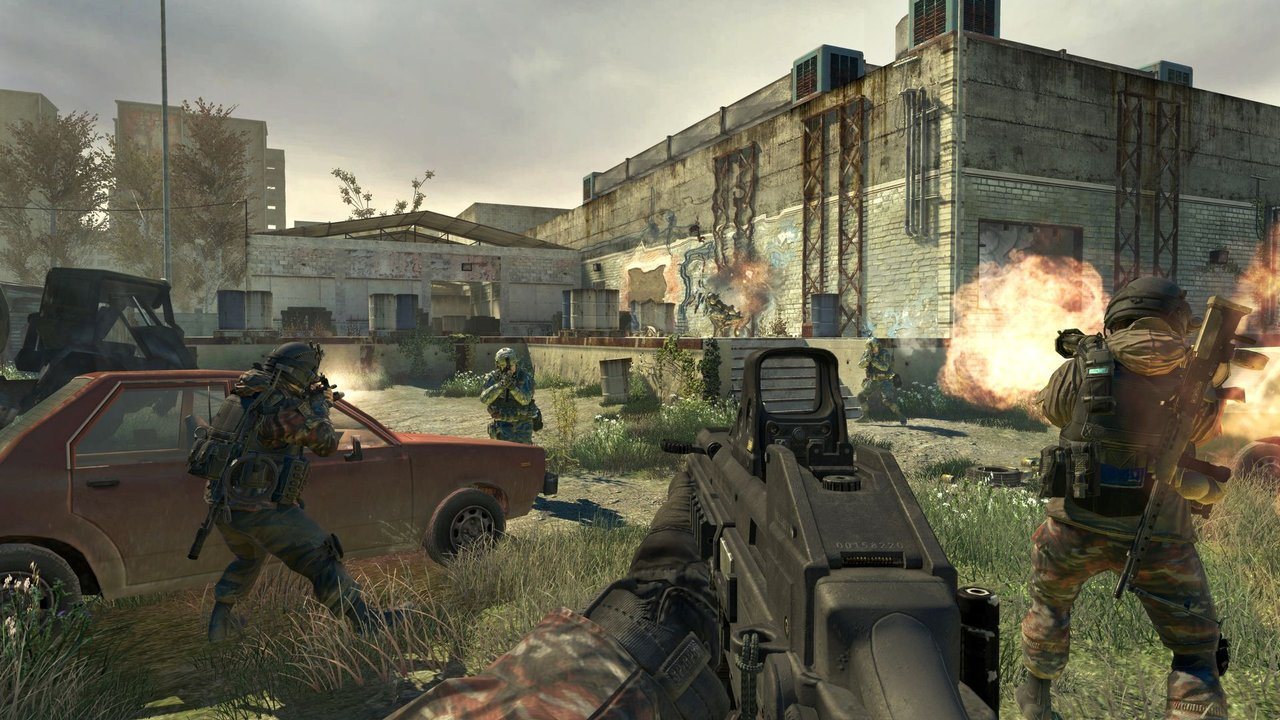
\includegraphics[scale=0.2]{img/codmw2.jpg}
	\end{center}
	
	\begin{center}
		Serán como los que hacemos en clase...
	\end{center}	
\end{frame}


\begin{frame}
	\frametitle{Probablemente sean así}

	\begin{center}
	Robinson 2.0
	
	    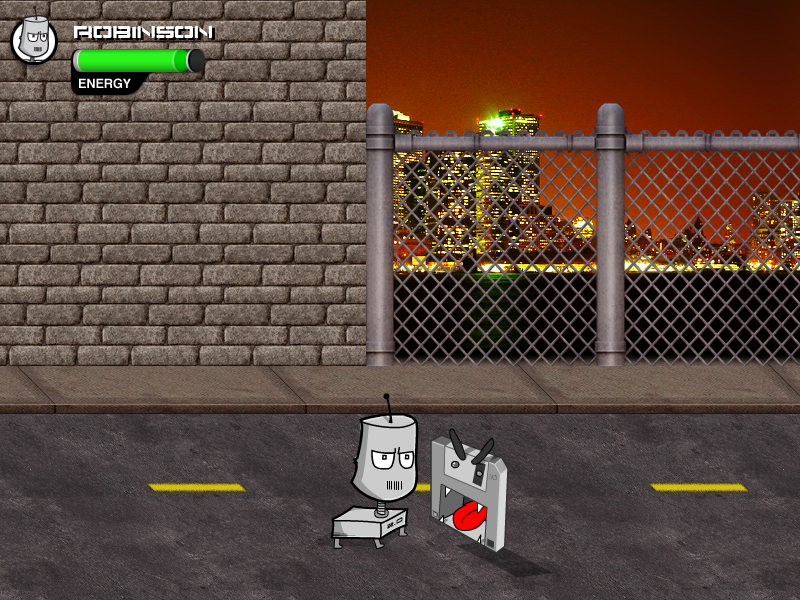
\includegraphics[scale=0.26]{img/robinson.png}
	    
	http://robinson.forja.rediris.es
	\end{center}
\end{frame}

\begin{frame}
	\frametitle{Probablemente sean así}

	\begin{center}
	Space Penguin
	
	    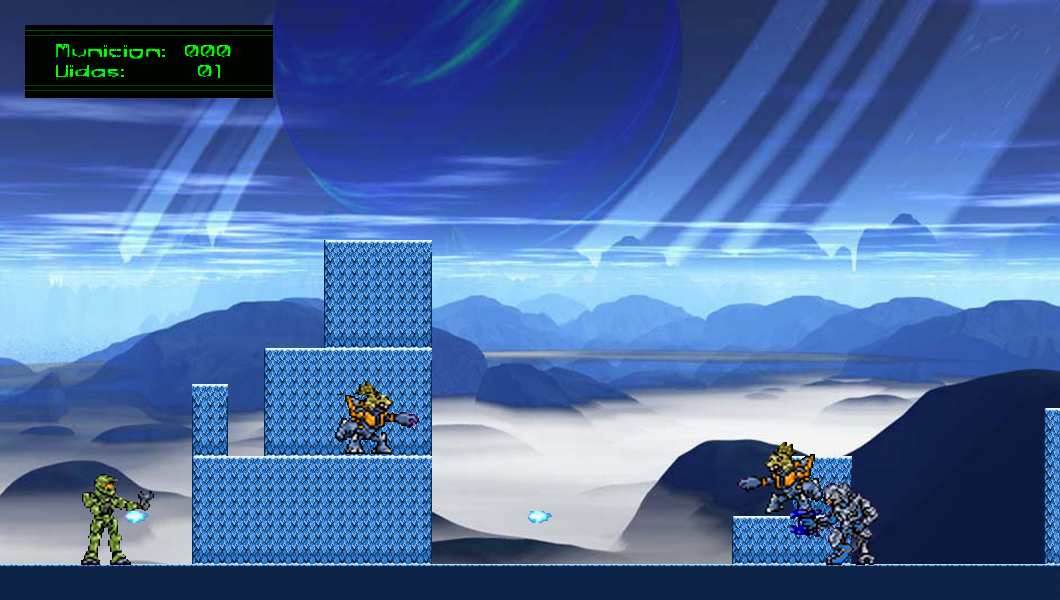
\includegraphics[scale=0.26]{img/spacepenguin.png}
	    
	http://spacepenguinproject.wordpress.com
	\end{center}
\end{frame}

\begin{frame}
	\frametitle{Probablemente sean así}

	\begin{center}
	Granny's Bloodbath
	
	    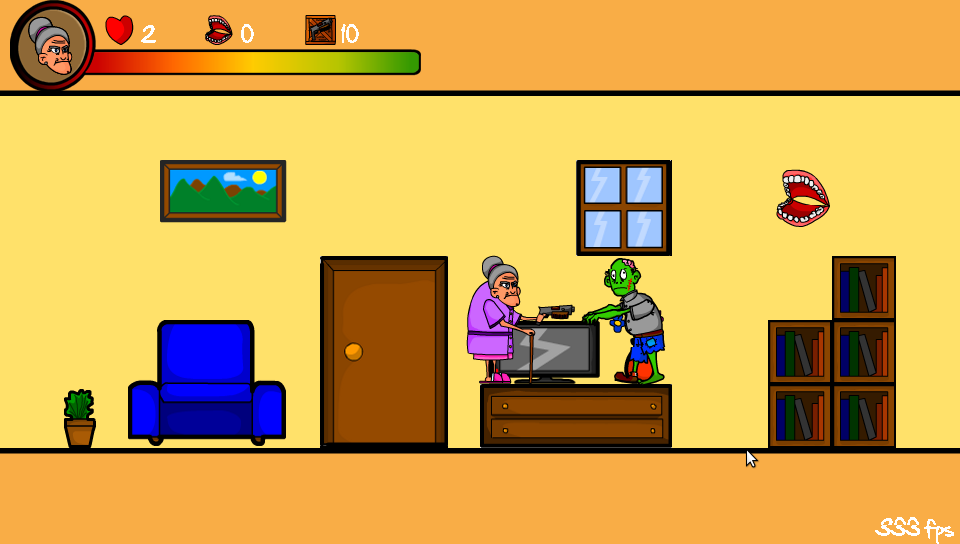
\includegraphics[scale=0.26]{img/grannysbloodbath.png}
	    
	http://grannysbloodbath.wordpress.com
	\end{center}
\end{frame}

\begin{frame}
	\frametitle{Probablemente sean así}

	\begin{center}
	Magic Duel
	
	    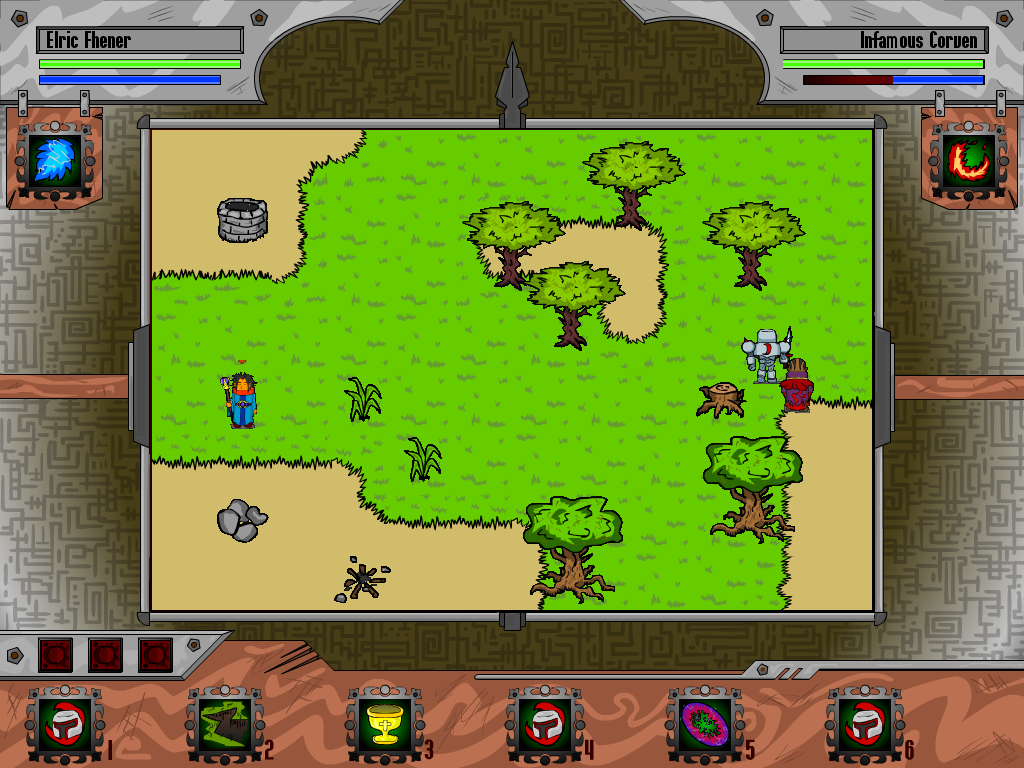
\includegraphics[scale=0.22]{img/magicduel.png}
	    
	http://meydey.es/magicduel
	\end{center}
\end{frame}

\begin{frame}
	\frametitle{Diseño}
	
	\begin{center}
		Antes de lanzarse a programar hay que diseñar el juego
	\end{center}	
	
	\begin{columns}
	
	\column{175pt}
	\begin{block}{Modelado del mundo}
		\begin{itemize}
			\item Planteamiento y concepto
			\item Género
			\item Mecánicas
			\item Estructura de los niveles
			\item Personajes, enemigos y objetos
			\item Público objetivo
		\end{itemize}            
	\end{block}
	
	
	\column{125pt}
	\begin{center}
		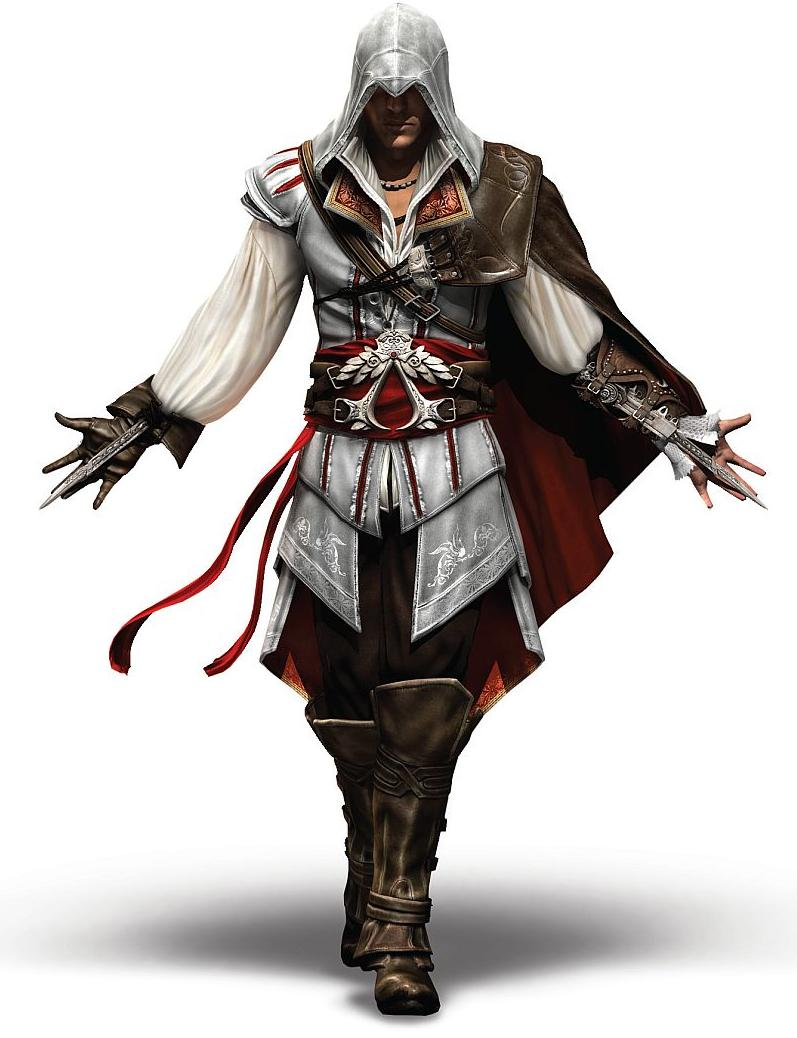
\includegraphics[scale=0.2]{img/assassins.jpg}
	\end{center}	
	
	
	\end{columns}
\end{frame}


\begin{frame}
	\frametitle{Game Loop}
	
	\begin{center}
		Todos los juegos siguen esta estructura, \textbf{\emph{Game Loop}}:
	\end{center}	
	
	\begin{columns}
	
	\column{125pt}
	\begin{center}
		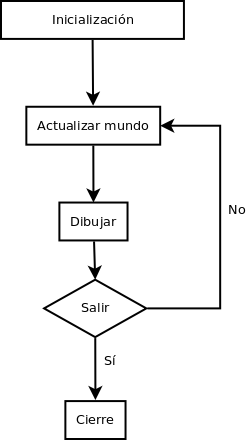
\includegraphics[scale=0.25]{img/gameloop.png}
	\end{center}	
	
	\column{175pt}
	\begin{alertblock}{Frames y movimiento}
		\begin{itemize}
			\item \emph{Actualizar}: los elementos reaccionan a su entorno y al usuario.
			\item \emph{Dibujar}: la escena se dibuja en pantalla.
			\item Si cada segundo se producen 25 iteraciones (25fps), tendremos sensación de movimiento.
			\item Guardamos los elementos del juego en variables.
		\end{itemize}            
	\end{alertblock}
	
	\end{columns}
\end{frame}

\begin{frame}
	\frametitle{Game Loop - Inicialización}
	
	Durante la etapa de inicialización se llevan a cabo las siguientes
	tareas:
	
	\begin{columns}[c]
	\column{200pt}
		
	\begin{block}{Pasos}
		\begin{itemize}
			\item Inicializar el motor y las librerías que usemos
			\item Cargar ficheros de configuración
			\item Dejar todo listo para empezar a trabajar
		\end{itemize}            
	\end{block}
	
	\column{100pt}
	
	\begin{center}
		
\includegraphics[scale=0.25]{img/engine.png}
	\end{center}	
	
	\end{columns}
	
\end{frame}

\begin{frame}
	\frametitle{Game Loop - Actualizar}
	
	Cada vez que actualizamos tenemos en cuenta:
	
	\begin{columns}[c]
	\column{175pt}
		
	\begin{block}{Actualizar}
		\begin{itemize}
			\item Entrada del usuario
			\item Red
			\item Movimiento y acciones del/los personaje/s
			\item Movimiento y acciones del/los enemigo/s, Inteligencia Artificial
			\item Colisiones, física
			\item Eventos aleatorios o asíncronos
		\end{itemize}            
	\end{block}
	
	\column{125pt}
	
	\begin{center}
		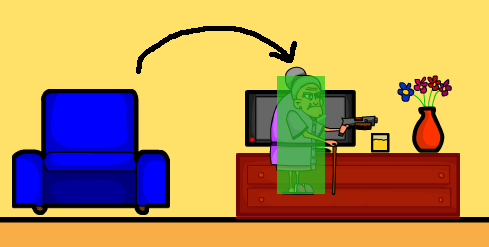
\includegraphics[scale=0.25]{img/grannycolision.png}
	\end{center}	
	
	\end{columns}
	
\end{frame}

\begin{frame}
	\frametitle{Game Loop - Dibujar}
	
	La fase de dibujado en un juego 2D:
	
	\begin{columns}[c]
	\column{175pt}
		
	\begin{block}{Dibujar}
		\begin{itemize}
			\item Dibujamos por capas, como The Gimp o Photoshop
			\item Componemos la escena por piezas
			\item Suele hacerse en orden (lejano-cercano)
			\item Algunas librerías permiten z-order
		\end{itemize}            
	\end{block}
	
	\column{125pt}
	
	\begin{center}
		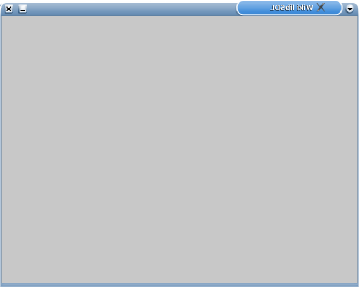
\includegraphics[scale=0.4]{img/pantalla.png}
		
		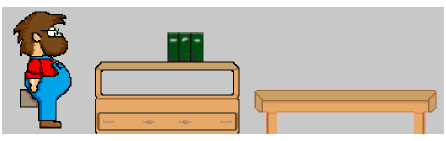
\includegraphics[scale=0.4]{img/elementos.png}
		
		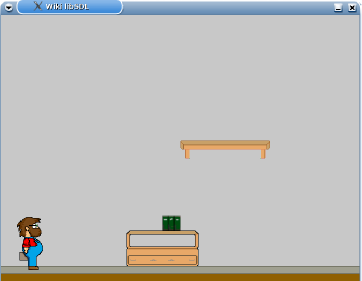
\includegraphics[scale=0.4]{img/composicion.png}
	\end{center}	
	
	\end{columns}
	
\end{frame}

\begin{frame}
	\frametitle{Game Loop - Cierre}
	
	¡Hay que recoger antes de salir!
	
	\begin{columns}[c]
	\column{175pt}
		
	\begin{block}{Cierre}
		\begin{itemize}
			\item Liberar todos los elementos del juego
			\item Cerrar las librerías en uso
			\item ¡Prevén las fugas de memoria!
		\end{itemize}            
	\end{block}
	
	\column{125pt}
	
	\begin{center}
		
\includegraphics[scale=0.6]{img/tidy.jpg}
	\end{center}	
	
	\end{columns}
	
	\begin{center}
	    ¡Los descuidos de memoria son muy peligrosos!
	\end{center}
	
\end{frame}
